% Chapter 1

\chapter{Introduction} % Write in your own chapter title
\label{Chapter1}
\indent Surveillance systems are ubiquitous and find many applications.
Existing video surveillance systems are still largely manual.
Normally, a surveillance camera sends video to a monitoring base
station, where it is monitored by a person or a group of people. Such an
arrangement is not foolproof, because it needs continuous manual
observation.  Any attempt in the direction of its automation can be of
great use in application areas such as:
\begin{itemize}
	 \item  Traffic Monitoring
	  \item Elderly care
	    \item Security
	    \item Monitoring of troops
\end{itemize}
\indent Moreover, an increasing number of video sources rely on resource
constrained (bandwidth-limited, delay-tolerant) networks.  Therefore,
there is a pressing need to evolve methods for conserving bandwidth
while the video data is transported from the point of acquisition to the
point of observation.\\ 
\indent A delay tolerant network(DTN) architecture lacks continuous end
to end connectivity. It works under some constraints like long delays
and extreme losses. For example, a military network having large number
of nodes with high data mobility in extreme environmental terrestrial
conditions is a DTN network. Such network normally employs their own
tailored routing algorithm for high throughput based on a individual
environmental conditions~\cite{1}. Smart home applications uses Zigbee,
DASH7 which are also DTNs.\\
\indent Zigbee and DASH7 networks have data rate of 200-250Kbits/sec.
With such networks at layer 1 and 2, there is tremendous need to conserve /
preserve the bandwidth needed by each video stream / all video streams
collectively.\\
\indent Video surveillance system can be integrated with existing home
network, but it is very important to achieve, reduction in amount of
data to be transmitted due to lack of end to end connectivity. A low
data rate node also allow the system to remain in sleep mode for longer
durations and hence prolongs longer battery life. Therefore a method
will be very useful by which, a few pre-processing operations allow us to
still carry out the primary objective - surveillance - while achieving
large and impressive savings on the required bandwidth.\\
\indent  For such implementation, it would be wise to transmit feature
information only. We need to extract this feature information out of
image and then send it over the network.  Ideally, we need to send the
minimum information about the image which allows us to reconstruct the
scenario or to detect an event. If possible then we need to detect the
event at the source node itself and then to transmit only this event
information over the DTN network.\\
\indent The end goal of such an intelligent system would be to offer an
automatic analysis of scene and then to infer desired information out of
it. These systems can be complex because of the complexity of the scene,
specially when application is targeted for outdoor monitoring.  Sometime
background of the scene can move, while in some other scene ambient
light can be different. Detection of foreground objects becomes a
non-trivial task.  Once we have foreground objects, we can save a lot of
bandwidth if we can detect if object has any significance of our
interest or not.\\
\indent A typical network of such system has been shown in
Fig.~\ref{KE}. Each Node can have a camera, a wireless transmission
module and a processing engine. Captured Image is processed to extract
semantic information (represented as text tags). Textual semantic
information is transmitted over the wireless media to the knowledge
engine. Knowledge engine uses ontology language to represent this
information from different nodes.
\begin{figure}[!b]
\centering
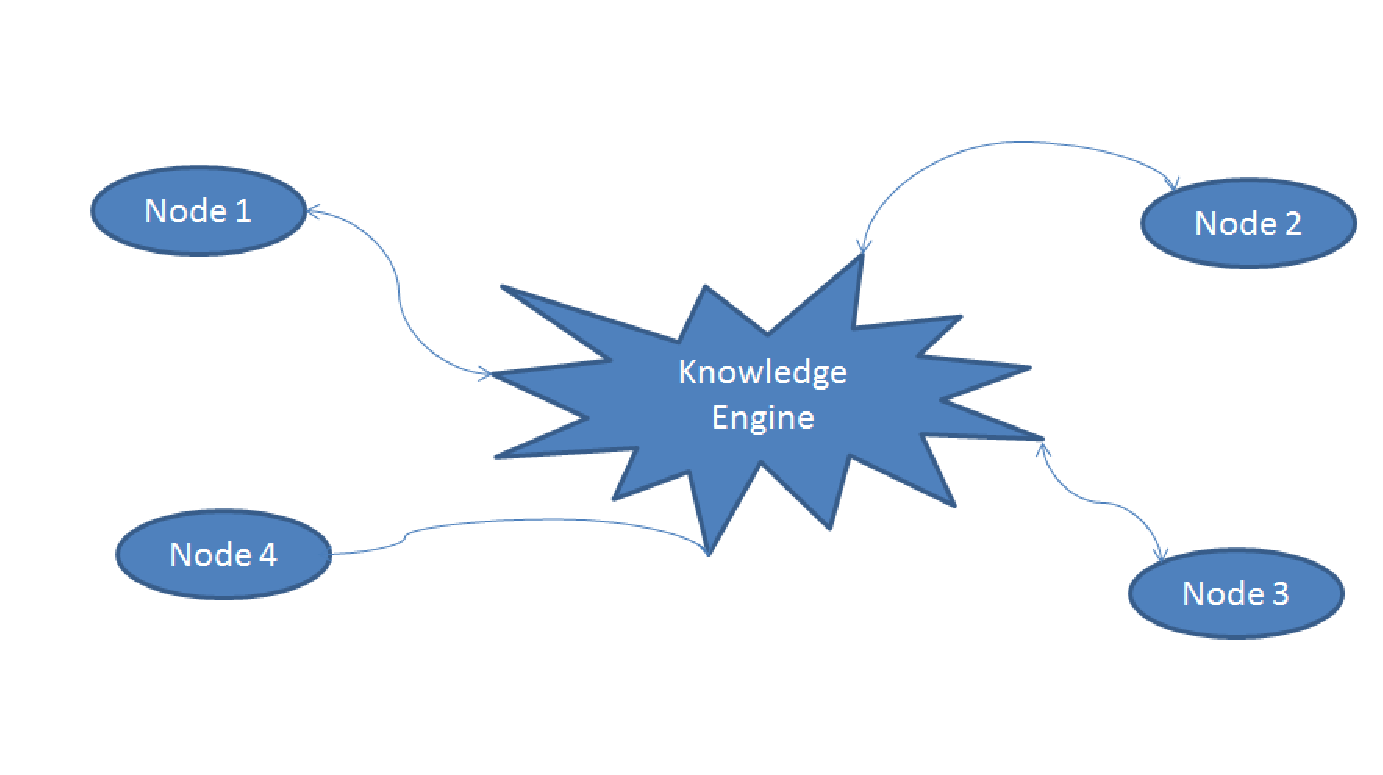
\includegraphics[height=200pt]{Figures/KE}
\caption{Surveillance camera network}
\label{KE}
\end{figure}

\indent \textbf{Problem statement:} We intend to detect moving person
and then to send only its feature information such as location, time of
detection etc to the monitoring station. Only sending such event
information would lead to design a ultra low bandwidth surveillance
system.  We want to keep our computation cost very low, at the same time
with high genuine detection rate and low false detection rate. We also
want to run this application on low power CPU like ARM and to evaluate
the performance.
\section{Past Work and Literature Survey}
\subsection{Image transfer over delay tolerant / Low bandwidth networks}
\indent There has been no data available for the image transfer over
terrestrial DTNs, however there has been several attempts~\cite{2, 3,
4, 5} to transfer image over low bandwidth wireless sensor networks
(WSN). Zigbee is the most commonly used WSN protocol. It is based on
IEEE 802.15.4 standard which is mainly suited for low power home
network. Its power requirement is in range of 125-400 $\mu$W and data
rate is 250 Kbps.\\
\indent Pekhteryev et al.~\cite{2} have tried to transfer different
versions of JPEG images over Zigbee network and compared their
performance. This work shows that there is an effect of compression
coding algorithm on peak signal to noise ratio(PSNR). It has been
observed that compression technique with scalable coding is more error
tolerant in WSN environment. Hengstler et al.~\cite{3, 5} have used 3
cameras. One high resolution camera and two low resolution cameras. Low
resolution cameras have been used for stereo matching and to identify
any moving object in the camera's field of view (FOV). If a moving
object is found then only high resolution camera is triggered. Such a
system is power efficient in  comparison to the camera mote continuously
transmitting JPEG frames. Philips research laboratory had conceived idea
of xetal by putting CMOS image sensors and image processing logic on a
single integrated circuit. Wu et al.~\cite{4} have used xetal parallel
processors for image processing. After subtracting the background,
ellipse fitting has been done on the foreground object. This elliptical
information is collected from different camera and the 3D view is
reconstructed from it.

\begin{figure}[!b]
\centering
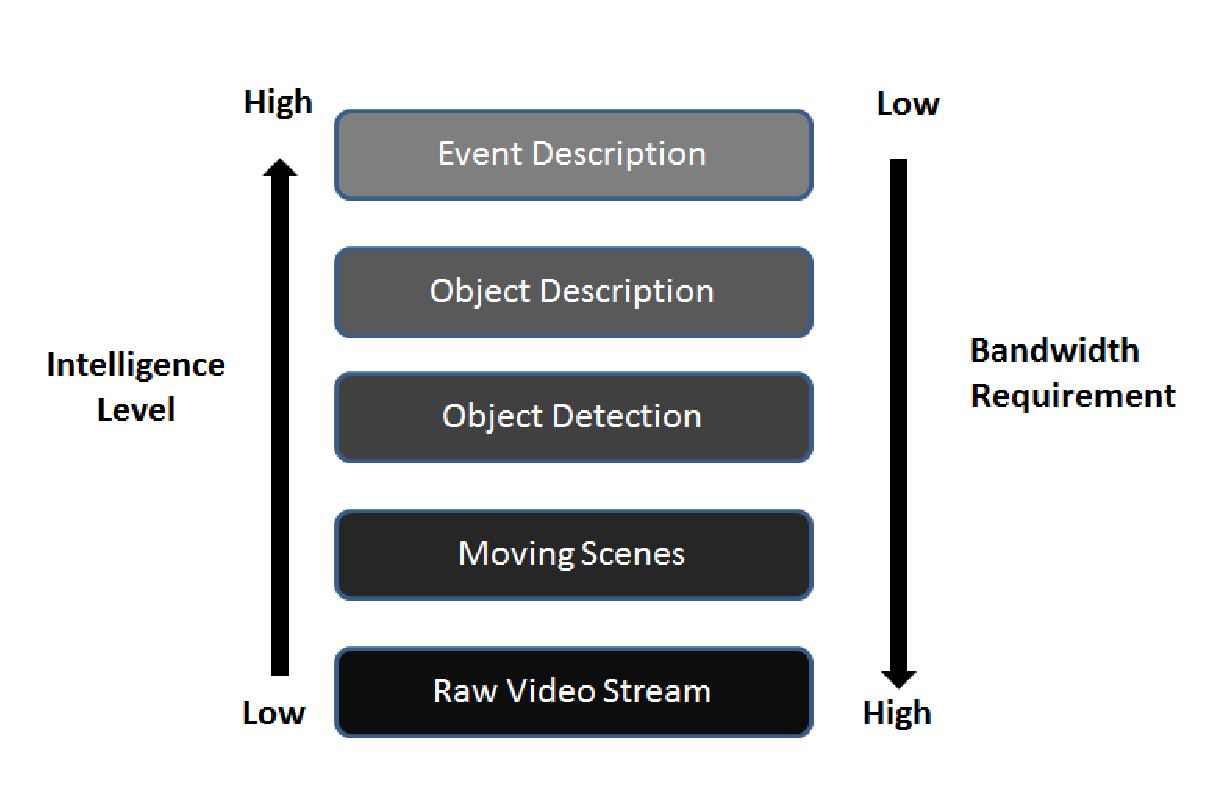
\includegraphics[height=300pt]{Figures/image_tr_level}
\caption{Surveillance image transfer level, reproduced from~\cite{3}}
\label{image_tr_level}
\end{figure}
\indent Fig.~\ref{image_tr_level} shows different level of
intelligence at which data can be transmitted in an augmented video
surveillance system. As we go above in the hierarchy, we attain higher
level of intelligence and save lot of bandwidth. But this is achieved at
the cost of increased computational power required at the mote node.
\subsection{Image size reduction techniques}
\indent Most of the image intensity information is not distinguishable
by human eye, so it is not relevant. Normally, neighbouring pixels of
the image are co-related to each other, so they are redundant. Such
redundancy is called spatial redundancy. Video may be thought of as a
large number of still images, which have been taken at very short
intervals of time. So, it is expected that there would be lot of
temporal redundancy between two neighbouring frames. Therefore an image
compression technique is developed around basic principal of reducing
irrelevancy and redundancy. Broadly, compression techniques are
categorised in lossless and lossy as explained by Shi et al. in his
book~\cite{6}. In a lossless compression, original image can be
retrieved exactly, but it does not give much compression.  Reconstructed
image after a lossy compression degrades in quality, however they
provide good amount of compression. We do not need to reconstruct exact
image for surveillance applications. So maximum possible compression
would reduce a lot of bandwidth on network.\\
\indent Most of the video coding methods are based on transform coding
followed by predictive coding based on motion estimation. Such methods
are called block based method, where prediction is implemented on a
complete block such as  MPEG-1,2. However, algorithms based
on object based coding techniques~\cite{7, 8} including MPEG-4 provides
substantially better compression. Chaudhury et al.~\cite{7} have used
principal component analysis (PCA) method for object
segmentation. Further, they have reused tracking subspace for object
coding which substantially reduced computational time. Babu et al.~\cite{8}
have calculated motion between current and previous frame.
Further, motion compensated error and other object parameters such as
boundary, location and motion information has been coded using suitable
source coding techniques.
\subsection{Background subtraction techniques}
\label{bg_subs_technique}
\indent In any object based method, the focus is on a foreground object
(FG) which is part of actual information. Simple way of getting FG
objects is to find difference with the previous frame. It is
computationally least expensive , but does not work for most of the
practical cases, unless following constraints are met.
\begin{itemize}
	\item Background is completely still.
	\item There is no variation in ambient light.
	\item Still camera has been used for image acquisition.
\end{itemize}
\indent Most background (BG) modeling algorithm find an image pattern
which does not have any moving object. However, this is a very complex
task, as sometimes camera itself might be moving, in some other cases
lighting condition can vary a lot. In some cases even all the moving
objects might not be of interest. For example, an escalator is the part
of BG in a scene where a person is standing on a moving escalator.\\
\indent Many methods~\cite{9, 10, 11, 12, 13, 14} have been developed
for the background subtraction (BGS), having strength and weakness in
terms of computation complexities and performance. Frame differencing is
of lowest computational complexity. The current frame is subtracted from
the last frame. If absolute value of resultant is less than a threshold
value, then that pixel is made part of BG.  The biggest drawback of this
method is that if an FG object stays for more than a frame time at any
position then that is made part of BG. Further, if an FG object consists
of almost uniformly distributed intensities, then internal portion of
the object is considered as BG. However, there is one advantage of this
method, it is quickly adaptable to the change in scene, as it depends on
only last frame.\\
\indent BGS algorithm~\cite{10, 12, 13, 14, 15} based on Gaussian
average or median of last couple of frames, comes in the category of
middle level of computational cost. Wren et al.~\cite{12} have used
running average of last n frames as BG model. Algorithms based on median
filter show better performance, but it requires more memory compared to
the running average method. Here, median of last n pixel is considered
as BG model.  McFarlane et al.~\cite{14} have used modified version as
average median filter, which has memory requirement same as that of
frame differencing.  Here, if a pixel value is greater than the
corresponding BG pixel, then BG pixel value is incremented by one, and
if it is less, then decremented by one.\\
\indent  Stauffer et al.~\cite{15} proposed to use Gaussian mixture
model (GMM) to create a background model. In this method, BG is
represented by Gaussian mixtures which is actually a probability that a
pixel value m is observed at time t. GMM works fine in removing BG
noise in multi-modal situations such as wavering tree. Since, it assumes
that BG is more frequently visible than the FG and , variance of BG is
significantly low, so it fails to adapt with sudden illumination
changes. It is also computationally very expensive.\\ 
\indent Yao et al.~\cite{11} have used a method based on local texture
features represented by local binary patterns (LBP) and photometric
invariant color measurements in RGB color space. Texture is an important
characteristic of images and video. LBP is invariant to any monotonic
gray level change.  LBP operator labels image pixel of a cell by
thresholding the neighborhood of each pixel with the center value and
considering the result as a binary number.\\
\indent LBP binary code of a pixel is calculated as follows:
\begin{equation}
LBP_{NR} = \Sigma _{n = 0} ^{N - 1} f(I_c - I_n) 2^n \hspace{20 mm} \mathrm{where} f(x) = \left\{ 
  \begin{array}{l l}
     1 & \quad \text{if $x$ $\geq$  $0$}\\
     0 & \quad \text{otherwise}
   \end{array} \right.
\end{equation}
\indent Here, $I_c$ is the gray value of central pixel and $I_n$ are the gray
value of pixels at a distance of radius $R$.  On a multi channel color
image LBP can be calculated at each pixel separately. LBP works well with
local illumination changes, however there can be issues in case of
global illumination change. LBP fails when both background and foreground
of an image shares same texture information. Yao et al.~\cite{11} have used
photometric invariant color features in RGB color space to overcome this
limitation of LBP.\\
\indent Visual background extractor(Vibe)~\cite{9} is another important
implementation which need to be discussed before completing this
section. There is a common strategy to use first in first out method to
update background model. Large number of samples is included in the
background model to cater varied events. However, computation time
increases with each increment in number of samples of background model.
Vibe has a unique way to overcome these issues. It decides about
background pixel value after comparison with closest samples selected
randomly. Say, $N$ is the number of samples corresponding to each
background pixel. One out of $N$ samples is selected
randomly and is replaced by current pixel value. Furthermore,
updated values of sample are diffused to their randomly selected
neighbouring pixel. Thus sample data base is created. Euclidean distance
is calculated between current pixel value and samples corresponding to
current pixel. If at least $m$ samples have euclidean distance less than
a threshold (say $T$), then that pixel is assigned to BG, else assigned to
FG.
\subsection{Object detection techniques}
\indent With the procedure discussed earlier in
section~\ref{bg_subs_technique}, we are able to reduce image size
significantly going with object centric methods. However, the output is
still an image. To reduce the output size further, this image data need
to be converted into information. We wish that our system is able to
answer question about the image data, such as, is there any moving
person in the image data? The first task for object detection from the
image is to extract features of the objects. These features could be
intensity, edges, color, size, texture, motion pattern, contour etc.
Most of the detection method works with two steps: (a) by preparing a
statistical model of training set images and then (b) comparing features
of test object with that of the model.  Training data set is prepared
using both positive and negative objects. Positive objects are those
true objects which have been targeted for detection, remaining other
objects are called negative objects. For example, if we target detection
of a moving human then, all moving human in scene will be labeled as
positive object and other moving objects such as vehicle, animal etc
will be labeled as negative object.\\
\indent Person Finder(PFinder) developed by Wren et.al~\cite{12} seems
first attempt to recognize human and its behavior in a practical
scenario. It works with Maximum A Posteriori Probability (MAP) method
for human detection and tracking. It uses color and shape based
descriptor for distinguishing different body parts such as hand and
head.\\
\indent The Viola and Jones $[VJ]$ method~\cite{16, 17} is equally
popular. Their method is based on Haar-like like features. To find these
features in any detection window, adjacent rectangular regions are
created at a specific location. Pixel intensities of each region is
added together and then difference of sum is calculated. This difference
is used as Haar-like feature descriptor. Further, the same authors have
provided new concept of image representation as integral image.  Pixel
value at any location in an integral image is sum of all the pixels
above and left of that pixel.  These can be computed with very few
operations per pixel.  Integral image representation helps in
computation of Haar-like like features in constant time.\\
\indent Work by Viola et al. in~\cite{17} was primarily used for
face detection.  Above work of $[VJ]$ with motion information was further
used for human detection in~\cite{16}.  AdaBoost has been used to
select a small set of features out of all Haar-like like features and to
train the classifier. They have used rectangular features which are
sensitive to edges, bars but are quite coarse. However, these features
in association with integral image provides sufficient compensation for
the above limitations. Jones et al.~\cite{26} have further improved
the performance of above method by using ten frames instead of two frames
for motion analysis. They divide detector into eight direction specific
detectors.\\
\indent In~\cite{20, 21}, it is shown that histogram of oriented
gradient (HOG) descriptor has better performance than Haar-like based
descriptors. Edge or gradient are very specific property of local shape.
An image is divided into small cells and histogram of edge / gradient
direction is calculated for each cell. This is called HOG descriptor.
Since this descriptor works with localised cells, therefore they are
invariant to geometric and photometric transformations. Further these
descriptors are fed to support vector machine(SVM) classifier for human
detection.\\
\indent In continuation of above method, Zhu et al.~\cite{20} did some
modifications for performance improvements. Instead of fixed size
blocks, they have used variable sized block and then AdaBoost has been
used to detect the best block suited for detection. They have used
integral image (a concept provided by $[VJ]$ in~\cite{17})for faster
computation of HOG features.\\
\indent Some work~\cite{30} have also been done for human motion
detection using multiple cameras. Multiple cameras allow depth view
calculation of different body parts, which assist further in
detection.\\
\indent Yao et al.~\cite{25} have used covariance feature with cascade
of logitboost classifier as human descriptor. Covariance matrix encodes
information about variance of features, their correlation with each
other, and special layout. Integral image concept is used here too for
faster computation. The covariance matrix $C_R$ of the features are
computed as follows:
\begin{equation}
\begin{aligned}
& C_R = {1 \over {(|R| - 1)}} \Sigma _{x \in R} (H(x) - m_R) (H(x) - m_R)^T\\
& m_R = {1 \over {(|R|)}} \Sigma _{x \in R} H(x)
\end{aligned}
\end{equation}
Where, $m_R$ is the mean vector in region R.\\
\indent Image skeletonization followed by motion pattern analysis is
computationally very fast way to detect a human. These authors~\cite{32,
22, 31} have used this method for human motion analysis. Change in
angle between legs is periodic. So an autocorrelation tells about cyclic
nature of angle between legs. However, autocorrelation induces noise due
to the DC bias of this angle signal. To overcome this issue, high
frequency pre-emphasis filter to the angle signal is applied before
autocorrelation operation. We have used similar method for human
detection in our approach with the slight variation at autocorrelation
steps, which allowed us to not go for pre-emphasis step and save
computation time.
\subsection{Outstanding issues}
\indent Methods based on Haar-like, HOG or covariance feature descriptor
works with even single image frame, however they are computationally
very slow and still not viable for low cost embedded applications.
Therefore further research is needed to optimize these methods to fit
into viable embedded applications. Skeletonization followed by motion
pattern analysis is not a generic method for all types of object
detection. However, it can be successfully used for moving human. It
seems that it has lower computational cost, which need to be evaluated.
These algorithm need to be tested with multiple frames having multiple
human. They also need to be tested with false moving objects. Complete
implementation need to be tested with a low cost embedded solution.
\section{Motivation}
\indent Low bandwidth along with low power augmented surveillance system
is going to be hot research area in coming years. Ultra low bandwidth
surveillance system will fit into ubiquitous low power delay tolerant
home network (such as Zigbee). So, the evaluation of all stages of
surveillance image / video processing which can cater such needs will be
a contribution in this direction. Overall it seems that there are two
important steps in the complete flow which need to be evaluated before
selecting final one for the proposed framework. We need to find
computationally efficient BGS algorithm. We also need to see that which
algorithm is suitable for pedestrian detection in embedded environment.
In our work, we will first evaluate few important BGS and human
detection algorithms. Wherever possible, we will try to optimize
the finally selected algorithm and will try to see if combined execution
time of all stages is suitable for an embedded application or not.
\section{Organisation of thesis}
\indent In chapter 1 we have discussed about important work done in the
area of background subtraction and human detection. We have also
discussed about outstanding issues and the issues which we are going to
address with our work.\\
\indent In chapter 2, we discuss in detail about how other authors
have done similar job. We also talk about our approach and
framework for a low bandwidth augmented surveillance system.\\
\indent In chapter 3, we provide details of embedded implementation of
our approach discussed in chapter 2.\\
\indent In chapter 4, we have analyzed the results obtained in our
approach. At the end we address remaining issues and direction for the
future work.
